
Insulation dimensions:

\begin{equation}
    A_\text{ins} = a^2 - \frac{\pi d_\text{strand}^2}{4}
\end{equation}

\begin{equation}
    p_\text{avg} = \frac{4 a + \pi d_\text{strand}}{2} 
\end{equation}

\begin{equation}
    L_\text{ins} = \frac{A_\text{ins}}{p_\text{avg}}
\end{equation}

\begin{equation}
    A_\text{ins,cond} = \frac{\frac{1}{4} A_\text{ins} ~ L_{winding}}{L_\text{ins}}
\end{equation}

\begin{figure}[H]
\centering
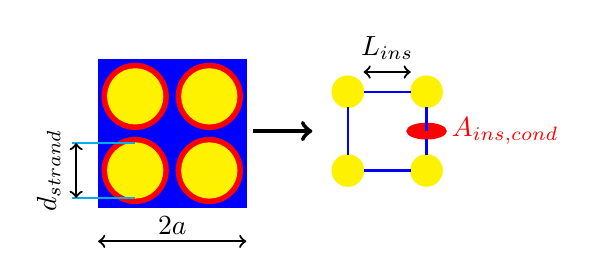
\begin{tikzpicture}[scale = 1]
\filldraw[blue] (-0.941/2,-0.941/2) rectangle (0.941/2,0.941/2);
\filldraw[red] (0,0) circle (0.7/2+0.07);
\filldraw[yellow] (0,0) circle (0.7/2);
\filldraw[blue] (-0.941/2,-0.941/2+0.941) rectangle (0.941/2,0.941/2+0.941);
\filldraw[red] (0,0+0.941) circle (0.7/2+0.07);
\filldraw[yellow] (0,0+0.941) circle (0.7/2);
\filldraw[blue] (-0.941/2+0.941,-0.941/2) rectangle (0.941/2+0.941,0.941/2);
\filldraw[red] (0+0.941,0) circle (0.7/2+0.07);
\filldraw[yellow] (0+0.941,0) circle (0.7/2);
\filldraw[blue] (-0.941/2+0.941,-0.941/2+0.941) rectangle (0.941/2+0.941,0.941/2+0.941);
\filldraw[red] (0+0.941,0+0.941) circle (0.7/2+0.07);
\filldraw[yellow] (0+0.941,0+0.941) circle (0.7/2);
\draw[thick, cyan] (-0.8,0.7/2) -- (0,0.7/2);
\draw[thick, cyan] (-0.8,-0.7/2) -- (0,-0.7/2);
\draw[black, thick, <->] (-0.75,0.7/2) -- (-0.75,-0.7/2);
\node[scale = 1, rotate=90] at (-1.1, 0) {$d_\text{strand}$};
\draw[thick,<->] (-0.941/2,-0.9) -- (0.941*1.5,-0.9);
\node[scale = 1] at (0.941*0.5, -0.7) {$2a$};
\draw[ultra thick,->, black] (1.5,0.5) -- (2.25,0.5);
\filldraw[yellow] (2.7,0) circle (0.2);
\filldraw[yellow] (3.7,0) circle (0.2);
\filldraw[yellow] (3.7,1) circle (0.2);
\filldraw[yellow] (2.7,1) circle (0.2);
\draw[thick, blue] (2.9,0) -- (3.5,0);
\draw[thick, blue] (2.9,1) -- (3.5,1);
\draw[thick, blue] (2.7,0.8) -- (2.7,0.2);
\filldraw[red] (3.7,0.5) ellipse (0.25cm and 0.1cm);
\draw[thick, blue] (3.7,0.8) -- (3.7,0.5);
\draw[thick, blue] (3.7,0.4) -- (3.7,0.2);
\draw[thick, black, <->] (2.9,1.25) -- (3.5,1.25);
\node[scale = 1] at (3.2, 1.55) {$L_\text{ins}$};
\node[scale = 1, red] at (4.7, 0.5) {$A_\text{ins,cond}$};
\end{tikzpicture}
\caption{Cross-sectional of 2D and 1D element}
\end{figure}